\documentclass[12pt,a4paper,fleqn]{article}
\usepackage[english]{babel}
\usepackage[utf8]{inputenc}
\usepackage[T1]{fontenc}
\usepackage{amsfonts}
\usepackage{amsmath}
\usepackage{amssymb}
\usepackage{amsthm}
\usepackage{graphicx}
\usepackage[left=2cm, right=2cm, bottom=3cm, top=2cm]{geometry}
\usepackage{float}
\usepackage{booktabs}
\usepackage{array}
\emergencystretch=2em
\usepackage{tikz}
\usetikzlibrary{arrows,positioning,shapes.geometric}


\newcommand{\N}{\mathbb{N}}
\newcommand{\R}{\mathbb{R}}
\newcommand{\SigmaGen}{\Sigma}
\newcommand{\id}{\operatorname{id}}
\newcommand{\UnifInt}{\operatorname{UnifInt}}
\newcommand{\Bern}{\operatorname{Bern}}
\newcommand{\card}{\operatorname{card}}
\newcommand{\clip}{\operatorname{clip}}
\newcommand{\ind}[1]{\mathbf{1}_{\{#1\}}}

\newcounter{algoritmo}
\newcommand{\algoritmo}[1]{\refstepcounter{algoritmo}\paragraph{Algorithm \thealgoritmo. #1}}

\tikzset{
	flowblock/.style={rectangle, rounded corners=2mm, draw=black, thick, align=center, minimum width=3.3cm, minimum height=1cm, fill=gray!10},
	flowdecision/.style={diamond, draw=black, thick, aspect=2.0, align=center, inner sep=1pt, fill=gray!10, text width=2.7cm},
	flowline/.style={->, >=stealth, thick},
	flowsmall/.style={rectangle, rounded corners=1.5mm, draw=black, thick, align=center, minimum width=2.7cm, minimum height=0.8cm, fill=gray!10},
	tensornode/.style={circle, draw=black, thick, minimum size=4.2mm, inner sep=0pt, fill=white},
	inputnode/.style={circle, draw=black, thick, minimum size=4.2mm, inner sep=0pt, fill=green!25},
	outputnode/.style={circle, draw=black, thick, minimum size=4.2mm, inner sep=0pt, fill=red!25},
	internode/.style={circle, draw=black, thick, minimum size=4.2mm, inner sep=0pt, fill=blue!10},
	boxnote/.style={rectangle, rounded corners=2mm, draw=black, thick, align=left, fill=gray!8, inner sep=5pt}
}

\title{\textbf{Artificial Simulation of Neuronal Evolution}}
\author{F. Bottega}
\date{\today}

\begin{document}
\maketitle

\begin{abstract}
\noindent This article describes a computational model of digital organisms controlled by evolving artificial brains. Unlike traditional layer-based artificial neural networks, the proposed model represents each brain as a three-dimensional mesh of partially connected neurons, with topology, firing parameters, connectivity regions, and plasticity rules defined by a discrete genome. The organisms inhabit a two-dimensional environment, receive sensory signals, process those signals through a recurrent neuronal dynamics, and execute binary motor actions. Selection is not defined by an explicit loss function; it emerges from a simple ecology based on energy, feeding, survival, and reproduction. We present the formalization of the genome, the rules of phenotypic generation, the signal propagation dynamics, the plasticity of connections, the recombination mechanism through offspring, and the implementation methodology in Godot and Python via WebSocket. In addition to the formal description, the text emphasizes a didactic presentation of the system through flowcharts, diagrams, and tables, making the links between theory, algorithm, and implementation explicit.


\medskip
\noindent \textbf{Keywords:} neuroevolution, genetic algorithms, artificial agents, neuronal plasticity, agent-based simulation, complex systems.
\end{abstract}

\section{Introduction}

Traditional artificial neural networks are generally built from pre-specified architectures: layers, blocks, activation functions, matrix operations, and an objective function that guides parameter fitting. This approach is extraordinarily effective in many domains, but it imposes a strongly engineered computational structure. Even when the architecture is large and training is statistical, much of the shape of the cognitive system is defined before experience.

The goal of this work is to explore a complementary direction: to simulate digital organisms whose neuronal structures are not organized in layers, but in a three-dimensional, partially connected mesh that is genetically specified and can be plastically modified throughout life. The methodological hypothesis is not that such a model is immediately competitive with conventional artificial neural networks, but that it offers a suitable experimental space for investigating more organic forms of adaptation, recurrence, memory, self-organization, and environmental selection.

In this model, a digital organism, called here a \emph{blob}, has an artificial brain. The brain is defined by a discrete tensor
$$
	B = [a] \times [b] \times [c],
$$
where $[n]=\{0,1,\ldots,n-1\}$ and $a,b,c \in \N$. Each element of $B$ represents a neuron. Some neurons receive sensory signals, some are associated with motor actions, and the rest function as internal neurons. Connections between neurons are directional, not necessarily symmetric, and do not follow a layered structure.

The contribution of this text is to formalize the current prototype of the simulation. The article describes:

\begin{enumerate}
	\item the genetic representation used to generate artificial brains;
	\item the genotype--phenotype transformation;
	\item neuronal signal dynamics;
	\item the rules of structural plasticity and connection weakening;
	\item the offspring rules by genetic recombination;
	\item the implementation methodology in a Godot frontend and a Python backend.
\end{enumerate}

The current simulation should be understood as an exploratory prototype. In this version, there is no global scalar fitness function, gradient backpropagation, or supervised learning. Selective pressure is environmental: organisms that consume energy without finding food die; organisms that survive long enough and collide with other organisms may generate offspring.

\begin{figure}[H]
\centering
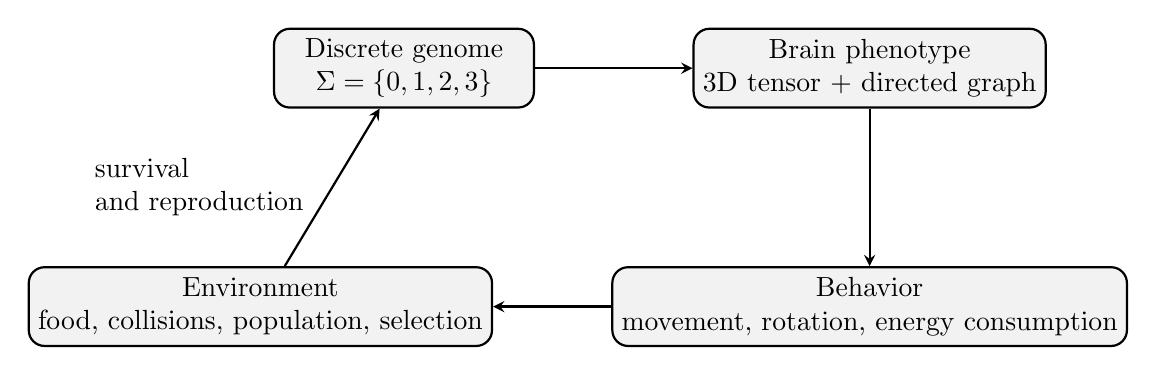
\begin{tikzpicture}[node distance=1.0cm]
	\node[flowblock] (genoma) {Discrete genome\\$\Sigma=\{0,1,2,3\}$};
	\node[flowblock, right=2.0cm of genoma] (fenotipo) {Brain phenotype\\3D tensor + directed graph};
	\node[flowblock, below=2.0cm of fenotipo] (comportamento) {Behavior\\movement, rotation, energy consumption};
	\node[flowblock, left=1.5cm of comportamento] (ambiente) {Environment\\food, collisions, population, selection};
	\draw[flowline] (genoma) -- (fenotipo);
	\draw[flowline] (fenotipo) -- (comportamento);
	\draw[flowline] (comportamento) -- (ambiente);
	\draw[flowline] (ambiente) -- node[left, align=left]{survival\\and reproduction \ \ } (genoma);
\end{tikzpicture}
\caption{Conceptual cycle of the model: the genome defines the brain, the brain produces behavior, behavior interacts with the environment, and the environment determines which genomes persist.}
\label{fig:ciclo-conceitual}
\end{figure}

\section{Initial definitions}

\subsection{Neuronal space}

Given dimensions $a,b,c$, the set of neurons is
$$
	V_{a,b,c} = [a] \times [b] \times [c].
$$
For implementation purposes, each neuron $(i,j,k) \in V_{a,b,c}$ is identified by a linear index
$$
	\alpha(i,j,k) = i + ja + kab.
$$
The set of neuron indices is therefore
$$
	\mathcal{V}_{a,b,c} = \{0,1,\ldots,abc-1\}.
$$
The inverse transformation is given by
$$
	x(n)= n \bmod a,\qquad
	y(n)= \left\lfloor\frac{n}{a}\right\rfloor \bmod b,\qquad
	z(n)= \left\lfloor\frac{n}{ab}\right\rfloor.
$$
Thus, when convenient, we identify neuron $n \in \mathcal{V}_{a,b,c}$ with the coordinate
$$
	\alpha^{-1}(n) = (x(n),y(n),z(n)).
$$

\begin{figure}[H]
\centering
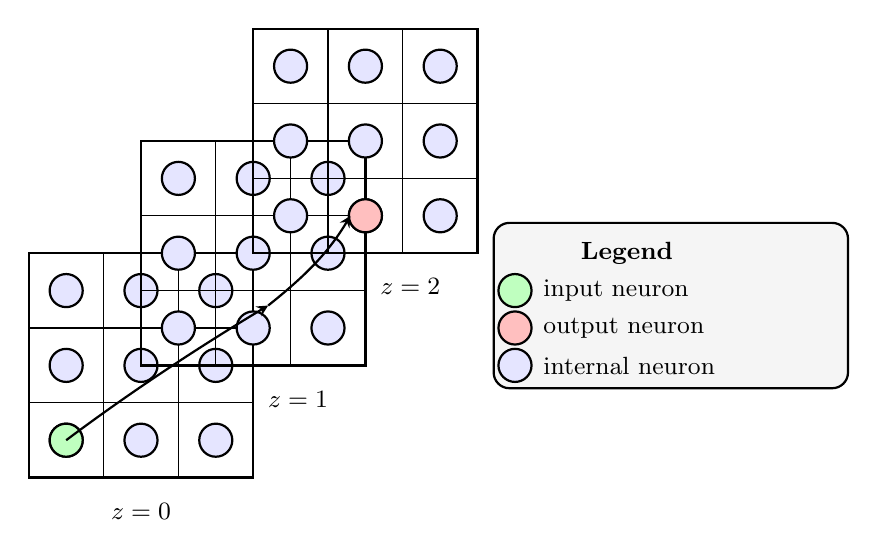
\begin{tikzpicture}[scale=0.95]
	\begin{scope}[shift={(0,0)}]
		\draw[thick] (0,0) rectangle (3,3);
		\foreach \x in {1,2}{\draw[thin] (\x,0)--(\x,3);}
		\foreach \y in {1,2}{\draw[thin] (0,\y)--(3,\y);}
		\foreach \i in {0.5,1.5,2.5}{\foreach \j in {0.5,1.5,2.5}{\node[internode] at (\i,\j) {};}}
		\node[font=\small] at (1.5,-0.45) {$z=0$};
	\end{scope}
	\begin{scope}[shift={(1.5,1.5)}]
		\draw[thick] (0,0) rectangle (3,3);
		\foreach \x in {1,2}{\draw[thin] (\x,0)--(\x,3);}
		\foreach \y in {1,2}{\draw[thin] (0,\y)--(3,\y);}
		\foreach \i in {0.5,1.5,2.5}{\foreach \j in {0.5,1.5,2.5}{\node[internode] at (\i,\j) {};}}
		\node[font=\small] at (2.1,-0.45) {$z=1$};
	\end{scope}
	\begin{scope}[shift={(3.0,3.0)}]
		\draw[thick] (0,0) rectangle (3,3);
		\foreach \x in {1,2}{\draw[thin] (\x,0)--(\x,3);}
		\foreach \y in {1,2}{\draw[thin] (0,\y)--(3,\y);}
		\foreach \i in {0.5,1.5,2.5}{\foreach \j in {0.5,1.5,2.5}{\node[internode] at (\i,\j) {};}}
		\node[font=\small] at (2.1,-0.45) {$z=2$};
	\end{scope}
	\node[inputnode] at (0.5,0.5) {};
	\node[outputnode] at (4.5,3.5) {};
	\draw[flowline] (0.5,0.5) .. controls (1.3,1.1) and (2.2,1.7) .. (3.2,2.3);
	\draw[flowline] (3.2,2.3) .. controls (3.7,2.7) and (4.0,3.0) .. (4.3,3.5);
	\node[boxnote, anchor=west, minimum width=4.5cm, minimum height=2.1cm] (legenda) at (6.2,2.3) {};
	\node[anchor=west, font=\small\bfseries] at (7.25,3.0) {Legend};
	\node[inputnode] at (6.5,2.5) {};
	\node[anchor=west, font=\small] at (6.75,2.5) {input neuron};
	\node[outputnode] at (6.5,2.0) {};
	\node[anchor=west, font=\small] at (6.75,2.0) {output neuron};
	\node[internode] at (6.5,1.5) {};
	\node[anchor=west, font=\small] at (6.75,1.5) {internal neuron};
\end{tikzpicture}
\caption{Didactic representation of a brain as a three-dimensional tensor. Each $z$-plane contains a grid of neurons; some neurons are specialized as inputs and outputs, while the others are internal. The arrows illustrate directional connections.}
\label{fig:tensor-cerebral}
\end{figure}

\subsection{Brain graph}

The brain of an organism is represented by a directed graph
$$
	G=(\mathcal{V}_{a,b,c},E),
$$
where $E\subseteq \mathcal{V}_{a,b,c}\times \mathcal{V}_{a,b,c}$ is the set of directed connections. If $(u,v)\in E$, neuron $u$ can send signals to neuron $v$.

Each connection $(u,v)$ has a synaptic strength
$$
	\varepsilon_{uv}(t)\in\R_{\ge 0}
$$
at discrete time $t$. Initially, all accepted connections start with strength $1$. During the simulation, this strength can increase or decrease according to the usage of the connection.

When a connection weakens below zero, it is removed from the graph. Thus, the brain is not static: its effective graph evolves during the life of the organism.

\subsection{Inputs, outputs, and signals}

Let $N_I$ be the number of inputs and $N_O$ the number of outputs. The input neurons form a list
$$
	I=(i_1,\ldots,i_{N_I}),
$$
and the output neurons form a list
$$
	O=(o_1,\ldots,o_{N_O}).
$$
The lists are required to have no repeated indices and, in the current prototype, input and output neurons must be distinct from each other. The internal signal state is stored as a sparse map
$$
	s_t:\mathcal{V}_{a,b,c}\to\R_{\ge 0},
$$
whose support is finite at each step.

The neuronal state at time $t$ is a sparse function
$$
	s_t:\mathcal{V}_{a,b,c}\to\R_{\ge 0}.
$$
By convention, if a neuron does not appear in the map, its signal is zero. The external input vector is
$$
	X_t=(X_t^1,\ldots,X_t^{N_I})\in\R_{\ge 0}^{N_I},
$$
and the output vector is
$$
	Y_t=(Y_t^1,\ldots,Y_t^{N_O})\in\{0,1\}^{N_O}.
$$

The saturation function used to normalize signals is
$$
	\sigma(x)=1-e^{-x/\kappa}.
$$
Here $\kappa$ is a genetically defined parameter that controls how quickly a signal saturates.

\begin{table}[H]
\centering
\caption{Basic objects of the model and their interpretation.}
\label{tab:objetos}
\begin{tabular}{p{2.6cm}p{4.2cm}p{7.2cm}}
\toprule
Object & Notation & Interpretation \\
\midrule
Brain & $B=[a]\times[b]\times[c]$ & three-dimensional mesh of neurons \\
Graph & $G=(\mathcal{V},E)$ & effective directed connectivity structure \\
Inputs & $I=(i_1,\ldots,i_{N_I})$ & neurons that receive sensory signals \\
Outputs & $O=(o_1,\ldots,o_{N_O})$ & neurons that determine motor actions \\
Neuronal signal & $s_t(u)$ & intensity stored in neuron $u$ at time $t$ \\
Synaptic strength & $\varepsilon_{uv}(t)$ & intensity of the directed connection $(u,v)$ \\
Internal threshold & $\theta_u$ & firing threshold of neuron $u$ \\
Output threshold & $\Theta^{out}_{o_r}$ & threshold for activating the action associated with $o_r$ \\
\bottomrule
\end{tabular}
\end{table}

\section{Genetic representation}

\subsection{Genetic alphabet}

The genome is defined over the discrete alphabet
$$
	\SigmaGen=\{0,1,2,3\}.
$$
Optionally, these symbols can be interpreted as
$$
	0\mapsto A,\qquad 1\mapsto T,\qquad 2\mapsto C,\qquad 3\mapsto G.
$$
This interpretation is only symbolic. In the implementation, genes are handled as integers in $\{0,1,2,3\}$.

Given a genetic word
$$
	w=(w_1,\ldots,w_m)\in\SigmaGen^m,
$$
the decimal conversion is defined as
$$
	D_m(w)=\sum_{\ell=1}^{m} w_\ell 10^{m-\ell}.
$$
Note that $D_m$ does not interpret the word as a number in base 4. It concatenates the symbols as decimal digits restricted to $0,1,2,3$. For example,
$$
	D_5(1,0,3,2,1)=10321.
$$

The map
$$
	\mu:\SigmaGen\to\{0.2,0.4,0.6,0.8\},\qquad
	\mu(q)=\frac{q+1}{5}
$$
will also be used.

This map converts a genetic symbol into one of the four phenotypic values used as thresholds and probabilities in the model.

\subsection{Global parameters}

The current implementation uses the constant parameters listed in Table \ref{tab:parametros}.

\begin{table}[H]
\centering
\caption{Global parameters of the current model.}
\label{tab:parametros}
\begin{tabular}{lll}
\toprule
Symbol & Value & Meaning \\
\midrule
$N_I$ & $16$ & number of sensory inputs \\
$N_O$ & $4$ & number of motor outputs \\
$D$ & $5$ & word length for input/output coordinates \\
$D_2$ & $2$ & word length for regions and local coordinates \\
$D_3$ & $6$ & word length for the decay gene \\
$D_4$ & $4$ & word length for the initial number of connections \\
$A_{\min},A_{\max}$ & $4,7$ & limits of the first brain dimension \\
$B_{\min},B_{\max}$ & $4,7$ & limits of the second brain dimension \\
$C_{\min},C_{\max}$ & $4,7$ & limits of the third brain dimension \\
\bottomrule
\end{tabular}
\end{table}

\subsection{Complete genome}

The genome of a newly generated organism can be written as
$$
	\mathcal{G}=
	(G_{\dim},
	G_I,
	G_O,
	G_{O,\theta},
	G_R,
	G_Q,
	G_E,
	G_P,
	G_\theta,
	G_\delta,
	G_\tau,
	G_\kappa,
	G_\omega).
$$
Each component encodes one part of the brain phenotype:

\begin{table}[H]
\centering
\caption{Genetic components and their associated phenotypes.}
\label{tab:genes}
\begin{tabular}{p{3.1cm}p{4.4cm}p{7.2cm}}
\toprule
Gene & Form & Associated phenotype \\
\midrule
$G_{\dim}$ & $\SigmaGen^{3\times D}$ & dimensions $(a,b,c)$ \\
$G_I$ & $\SigmaGen^{N_I\times 3D}$ & input neurons \\
$G_O$ & $\SigmaGen^{N_O\times 3D}$ & output neurons \\
$G_{O,\theta}$ & $\SigmaGen^{N_O}$ & output thresholds \\
$G_R$ & $\SigmaGen^{abc\times 3D_2}$ & local connectivity regions \\
$G_Q$ & $\SigmaGen^{D_4}$ & maximum number of initial candidates per neuron \\
$G_E$ & dictionary of words in $\SigmaGen^{3D_2}$ & candidates for initial connections \\
$G_P$ & $\SigmaGen^{abc}$ & probabilities of creating new connections \\
$G_\theta$ & $\SigmaGen^{abc}$ & neuronal firing thresholds \\
$G_\delta$ & $\SigmaGen^{D_3}$ & synaptic strength decay \\
$G_\tau$ & $\SigmaGen^{D_2}$ & post-firing inactivity period \\
$G_\kappa$ & $\SigmaGen^{D_2}$ & saturation factor of the exponential response \\
$G_\omega$ & $\SigmaGen^{D_2}$ & gene reserved for the weakened period \\
\bottomrule
\end{tabular}
\end{table}

The gene $G_\omega$ is kept in the specification because it already exists in the implementation, but its phenotype is not yet used in the current dynamics.

\begin{figure}[H]
\centering
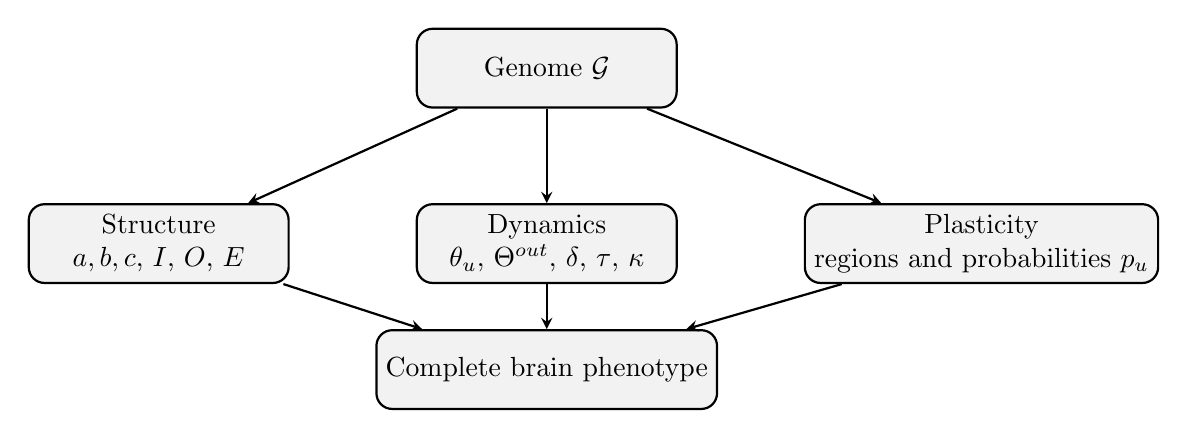
\begin{tikzpicture}[node distance=1.2cm]
	\node[flowblock] (g) {Genome $\mathcal{G}$};
	\node[flowblock, below left=1.2cm and 1.6cm of g] (estrut) {Structure\\$a,b,c$, $I$, $O$, $E$};
	\node[flowblock, below=1.2cm of g] (dinam) {Dynamics\\$\theta_u$, $\Theta^{out}$, $\delta$, $\tau$, $\kappa$};
	\node[flowblock, below right=1.2cm and 1.6cm of g] (plast) {Plasticity\\regions and probabilities $p_u$};
	\node[flowblock, below=2.8cm of g] (feno) {Complete brain phenotype};
	\draw[flowline] (g) -- (estrut);
	\draw[flowline] (g) -- (dinam);
	\draw[flowline] (g) -- (plast);
	\draw[flowline] (estrut) -- (feno);
	\draw[flowline] (dinam) -- (feno);
	\draw[flowline] (plast) -- (feno);
\end{tikzpicture}
\caption{Didactic decomposition of the genome into three functional groups: structural genes, dynamic genes, and plasticity genes.}
\label{fig:decomposicao-genoma}
\end{figure}

\section{Genetic rules for brain generation}

This section describes how a brain is built from a random genome. Generation is rejected and repeated when the structural constraints on inputs and outputs are not satisfied.

\subsection{Dimensions}

Let
$$
	G_{\dim}=
	\begin{pmatrix}
		g^a_1 & \cdots & g^a_D\\
		g^b_1 & \cdots & g^b_D\\
		g^c_1 & \cdots & g^c_D
	\end{pmatrix}.
$$
The brain dimensions are
$$
	a=\max\{A_{\min},\,D_D(g^a_1,\ldots,g^a_D)\bmod(A_{\max}+1)\},
$$
$$
	b=\max\{B_{\min},\,D_D(g^b_1,\ldots,g^b_D)\bmod(B_{\max}+1)\},
$$
$$
	c=\max\{C_{\min},\,D_D(g^c_1,\ldots,g^c_D)\bmod(C_{\max}+1)\}.
$$
In the current configuration, $a,b,c\in\{4,5,6,7\}$ and the number of neurons is
$$
	M=abc.
$$

\subsection{Genetic mapping to coordinates}

Given a word
$$
	w=(w^x,w^y,w^z)\in\SigmaGen^{3m},
$$
with blocks $w^x,w^y,w^z\in\SigmaGen^m$, define
$$
	\Phi_{a,b,c}^{(m)}(w)
	=
	\alpha\big(
	D_m(w^x)\bmod a,\,
	D_m(w^y)\bmod b,\,
	D_m(w^z)\bmod c
	\big).
$$
This function turns a genetic word into a neuron index.

\subsection{Input neurons}

For each input $r\in\{1,\ldots,N_I\}$, the row $G_I[r]$ defines
$$
	i_r = \Phi_{a,b,c}^{(D)}(G_I[r]).
$$
The input list is accepted only if
$$
	\card\{i_1,\ldots,i_{N_I}\}=N_I.
$$
If two inputs are mapped to the same neuron, the brain is rejected and a new genome is generated.

\subsection{Output neurons}

Similarly, for each output $r\in\{1,\ldots,N_O\}$,
$$
	o_r = \Phi_{a,b,c}^{(D)}(G_O[r]).
$$
The outputs are accepted only if
$$
	\card\{o_1,\ldots,o_{N_O}\}=N_O
$$
and
$$
	\{o_1,\ldots,o_{N_O}\}\cap\{i_1,\ldots,i_{N_I}\}=\varnothing.
$$
If either condition fails, the brain is rejected.

\subsection{Output thresholds}

Each output neuron receives a threshold
$$
	\Theta^{out}_{o_r} = \mu(G_{O,\theta}[r]).
$$
Thus,
$$
	\Theta^{out}_{o_r}\in\{0.2,0.4,0.6,0.8\}.
$$
When outputs are read, output $r$ is activated if
$$
	\sigma_\kappa(s(o_r))>\Theta^{out}_{o_r}.
$$

\subsection{Local connectivity regions}

Each neuron $u=\alpha(i,j,k)$ has a locally defined rectangular region determined genetically. Let $G_R[u]\in\SigmaGen^{3D_2}$ be split into three blocks. Define
$$
	R_x(u)=D_{D_2}(G_R^x[u])\bmod a,
$$
$$
	R_y(u)=D_{D_2}(G_R^y[u])\bmod b,
$$
$$
	R_z(u)=D_{D_2}(G_R^z[u])\bmod c.
$$
The nominal connectivity region of $u$ is
$$
	\mathcal{R}(u)=
	\left\{
		\alpha(p,q,r):
		|p-i|\leq R_x(u),\,
		|q-j|\leq R_y(u),\,
		|r-k|\leq R_z(u)
	\right\},
$$
with coordinates restricted to the bounds of the brain tensor.

The approximate biological interpretation is that each neuron has its own local reach. There is therefore no single global radius for the whole brain.

\subsection{Initial connections}

The gene $G_Q\in\SigmaGen^{D_4}$ determines the number of initial candidates per neuron:
$$
	Q = D_{D_4}(G_Q)\bmod(M-1).
$$
For each neuron $u=\alpha(i,j,k)$, $Q$ candidate words are generated
$$
	G_E[u,1],\ldots,G_E[u,Q]\in\SigmaGen^{3D_2}.
$$
Each candidate defines a possible destination
$$
	v_w=\Phi_{a,b,c}^{(D_2)}(G_E[u,w]).
$$
Connection $(u,v_w)$ is added if, and only if, the four conditions below are satisfied:
$$
	v_w\notin E(u),
$$
$$
	(v_w,u)\notin E,
$$
$$
	v_w\in\mathcal{R}(u),
$$
$$
	u\neq v_w \quad\text{or, if self-connection is allowed, it does not violate the other constraints.}
$$
In the current implementation, the explicit check prevents duplication and reverse connections; self-connections are not treated as a special case. The effective structure is the set of connections accepted after these filters.

\subsection{Probability of structural plasticity}

Each neuron receives a probability of creating new connections:
$$
	p_u=\mu(G_P[u])\in\{0.2,0.4,0.6,0.8\}.
$$
This parameter is used during the organism's life, when the neuron fires and tries to create a new connection with another active neuron in its region.

\subsection{Neuronal firing threshold}

Each neuron receives a firing threshold:
$$
	\theta_u=\mu(G_\theta[u])\in\{0.2,0.4,0.6,0.8\}.
$$
A neuron $u$ only propagates a signal when
$$
	s_t(u)>\theta_u
$$
and when it is not in its inactivity period.

\subsection{Synaptic decay}

The decay gene is a word
$$
	G_\delta=(d_1,\ldots,d_{D_3})\in\SigmaGen^{D_3}.
$$
Define
$$
	\delta = \sum_{\ell=1}^{D_3}d_\ell 10^{-\ell}.
$$
Equivalently, $\delta$ is the decimal number $0.d_1d_2\ldots d_{D_3}$. Since $d_\ell\in\{0,1,2,3\}$, in the current prototype $\delta$ lies in the interval
$$
	0\leq \delta \leq 0.333333.
$$
At each update, internal connections may have their strength reduced by
$$
	\delta^2.
$$

\subsection{Post-firing inactivity}

The inactivity period is
$$
	\tau=D_{D_2}(G_\tau)+1.
$$
This value defines the counter used to prevent a neuron from firing continuously in consecutive iterations. After firing, the neuron enters a refractory state controlled by this counter.

\subsection{Exponential factor}

The saturation function parameter is
$$
	\kappa=\left\lfloor\frac{D_{D_2}(G_\kappa)}{10}\right\rfloor +1.
$$
Since $D_{D_2}(G_\kappa)$ ranges from $0$ to $33$, it follows that
$$
	\kappa\in\{1,2,3,4\}.
$$

\subsection{Gene reserved for temporary weakening}

The gene
$$
	G_\omega\in\SigmaGen^{D_2}
$$
defines, in the current implementation, the value
$$
	\omega=\tau+D_{D_2}(G_\omega)+1.
$$
However, $\omega$ does not yet participate in the signal dynamics. It is kept as a reserved parameter for a possible extension in which neurons that have just fired would have a weakened period distinct from the inactive period.

\subsection{Genetic generation algorithm}

Algorithm 1. New brain generation

\begin{enumerate}
	\item Sample all genes of $\mathcal{G}$ independently and uniformly in $\SigmaGen$.
	\item Compute $(a,b,c)$ from $G_{\dim}$.
	\item Build the input neurons $I$ from $G_I$.
	\item If there is a collision between inputs, reject the genome and restart.
	\item Build the output neurons $O$ from $G_O$.
	\item If there is a collision between outputs, reject the genome and restart.
	\item If $I\cap O\neq\varnothing$, reject the genome and restart.
	\item Compute output thresholds, local regions, initial number of candidates, initial connections, plasticity probabilities, internal thresholds, decay, inactivity, and exponential factor.
	\item Initialize all neuronal signals as empty.
	\item Initialize all existing synaptic strengths as $1$.
	\item Initialize the inactivity counter of each neuron with value $\tau$.
	\item Return the symbolic genome $\mathcal{G}$ and the resulting brain phenotype.
\end{enumerate}

\begin{figure}[H]
\centering
\resizebox{\textwidth}{!}{%
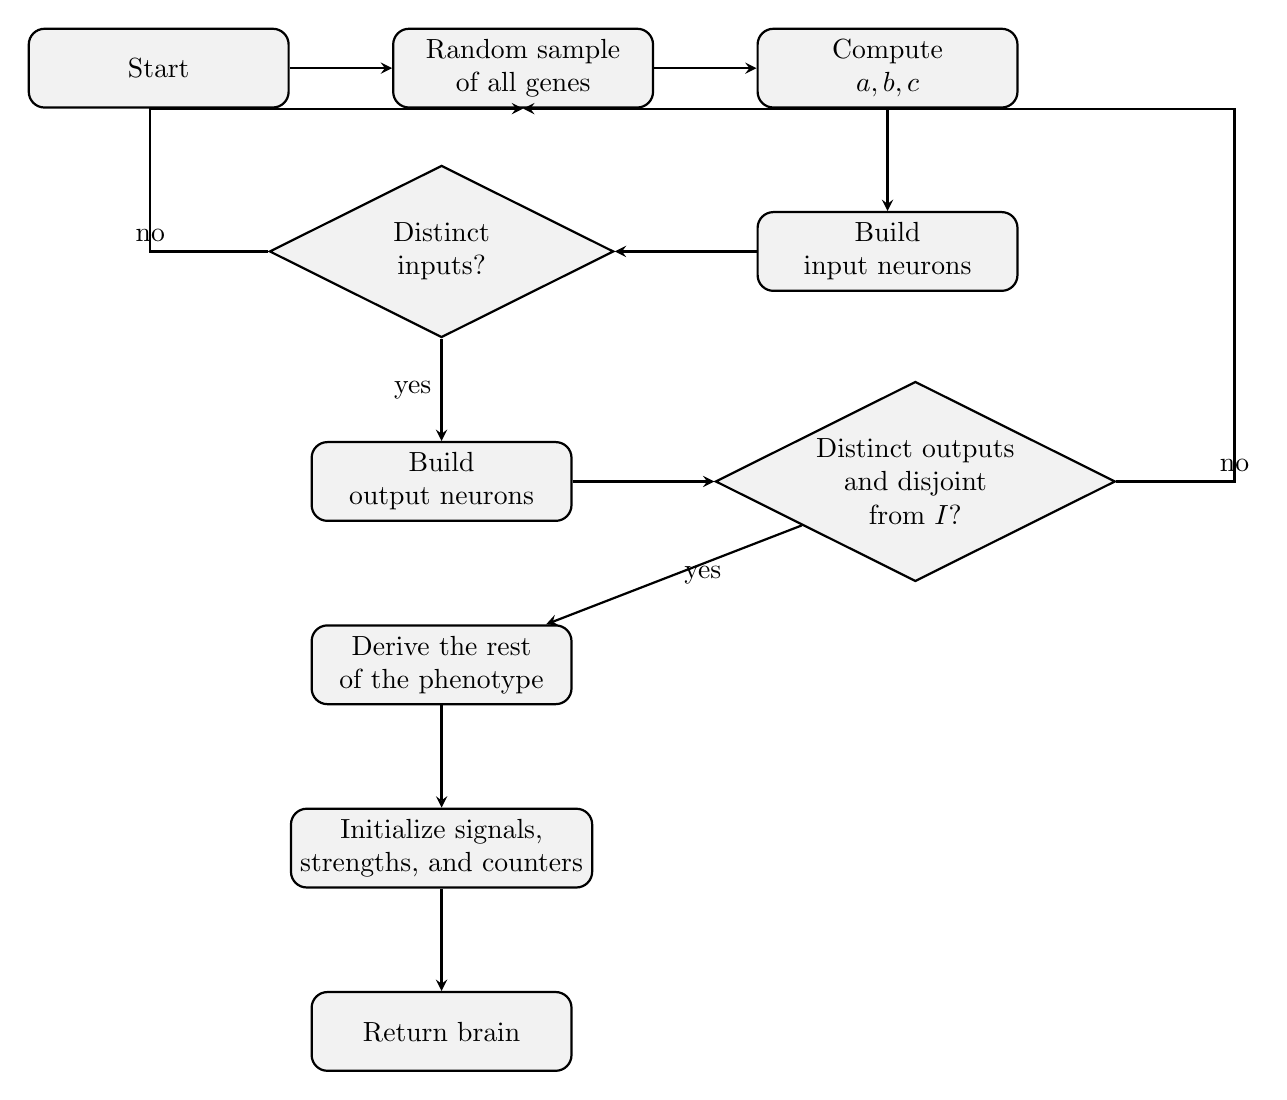
\begin{tikzpicture}[node distance=1.0cm and 1.0cm]
	\node[flowblock] (start) {Start};
	\node[flowblock, right=1.3cm of start] (sample) {Random sample\\of all genes};
	\node[flowblock, right=1.3cm of sample] (dims) {Compute\\$a,b,c$};
	\node[flowblock, below=1.3cm of dims] (inputs) {Build\\input neurons};
	\node[flowdecision, left=1.8cm of inputs] (din) {Distinct\\inputs?};
	\node[flowblock, below=1.3cm of din] (outputs) {Build\\output neurons};
	\node[flowdecision, right=1.8cm of outputs] (dout) {Distinct outputs\\and disjoint from $I$?};
	\node[flowblock, below=1.3cm of outputs] (resto) {Derive the rest\\of the phenotype};
	\node[flowblock, below=1.3cm of resto] (init) {Initialize signals,\\strengths, and counters};
	\node[flowblock, below=1.3cm of init] (end) {Return brain};

	\draw[flowline] (start) -- (sample);
	\draw[flowline] (sample) -- (dims);
	\draw[flowline] (dims) -- (inputs);
	\draw[flowline] (inputs) -- (din);
	\draw[flowline] (din) -- node[left]{yes} (outputs);
	\draw[flowline] (outputs) -- (dout);
	\draw[flowline] (dout) -- node[right]{yes} (resto);
	\draw[flowline] (resto) -- (init);
	\draw[flowline] (init) -- (end);
	\draw[flowline] (din.west) -- ++(-1.5,0) node[above]{no} |- (sample.south);
	\draw[flowline] (dout.east) -- ++(1.5,0) node[above]{no} |- (sample.south);
\end{tikzpicture}}
\caption{Flowchart of Algorithm 1. Genetic generation is a rejection-sampling procedure: whenever there is a collision between inputs or an invalid separation of inputs/outputs, the genome is discarded and a new one is sampled.}
\label{fig:fluxo-gen-brain}
\end{figure}

\section{Neuronal dynamics}

\subsection{State structure}

For each organism, the simulation keeps:

\begin{itemize}
	\item the set of connections $E_t$;
	\item the synaptic strengths $\varepsilon_{uv}(t)$;
	\item the neuronal signals $s_t(u)$;
	\item the inactivity counters $c_t(u)$;
	\item the current number of connections.
\end{itemize}

The processing of a neuronal step receives a vector of external inputs
$$
	X_t=(X_t^1,\ldots,X_t^{N_I})\in\R_{\geq 0}^{N_I}
$$
and returns a binary vector of outputs
$$
	Y_t=(Y_t^1,\ldots,Y_t^{N_O})\in\{0,1\}^{N_O}.
$$

\subsection{Propagation between neurons}

Consider a neuron $u$ with signal $s_t(u)>0$. It fires if
$$
	s_t(u)>\theta_u
$$
and
$$
	c_t(u)=\tau.
$$
When it fires, the effective transmitted signal is
$$
	\widehat{s}_t(u)=\sigma_\kappa(s_t(u)).
$$
For each connection $(u,v)\in E_t$, define the usage-updated strength:
$$
	\widetilde{\varepsilon}_{uv}(t)=\frac{1+\varepsilon_{uv}(t)}{2}.
$$
Then
$$
	\varepsilon_{uv}(t)\leftarrow \widetilde{\varepsilon}_{uv}(t)
$$
and neuron $v$ receives contribution
$$
	\Delta s(v) \leftarrow \Delta s(v)+\widetilde{\varepsilon}_{uv}(t)\widehat{s}_t(u).
$$
After transmitting, neuron $u$ is marked for zeroing:
$$
	s_{t+1}(u)\leftarrow 0,
$$
unless it receives another aggregated signal in the same step.

\subsection{Structural plasticity}

After a firing event, neuron $u$ tries to create a new connection. Let
$$
	\mathcal{C}_t(u)\subseteq\mathcal{R}(u)
$$
be a set of candidates sampled inside the local region of $u$. In the implementation, for computational economy, the search traverses a sample of approximately half of the points along each axis of the region instead of traversing the full region.

For each candidate $v\in\mathcal{C}_t(u)$, a new connection $(u,v)$ is created if:

$$
	U\leq p_u,\qquad U\sim \operatorname{Uniform}(0,1),
$$
$$
	v\in\operatorname{dom}(s_t),
$$
$$
	s_t(v)>0,
$$
$$
	(u,v)\notin E_t,
$$
$$
	(v,u)\notin E_t.
$$
When these conditions are satisfied,
$$
	E_{t+1}\leftarrow E_t\cup\{(u,v)\},
$$
$$
	\varepsilon_{uv}(t+1)=1.
$$
The rule creates at most one new connection per neuron firing.

\begin{figure}[H]
\centering
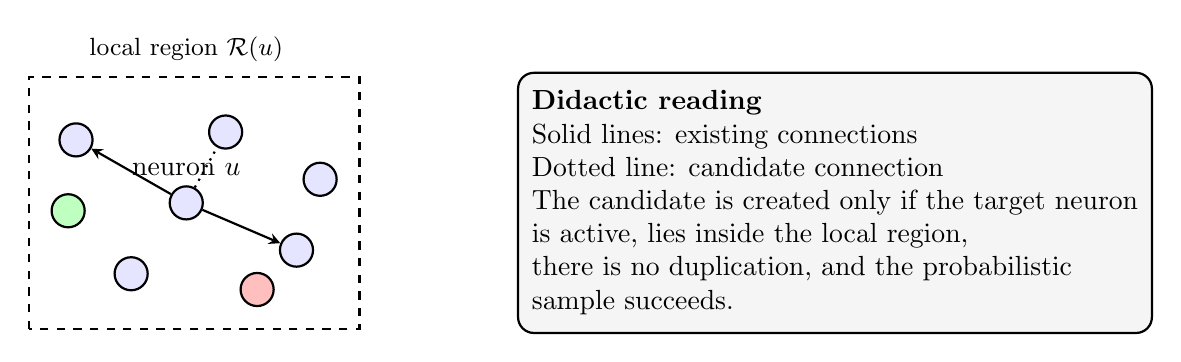
\begin{tikzpicture}[node distance=1.2cm]
	\node[internode, label=above:{neuron $u$}] (u) at (0,0) {};
	\draw[thick, dashed] (-2.0,-1.6) rectangle (2.2,1.6);
	\node[font=\small] at (0,1.95) {local region $\mathcal{R}(u)$};
	\foreach \x/\y/\name in {-1.4/0.8/a,-0.7/-0.9/b,0.5/0.9/c,1.4/-0.6/d,1.7/0.3/e}{
		\node[internode] (\name) at (\x,\y) {};
	}
	\node[inputnode] (iin) at (-1.5,-0.1) {};
	\node[outputnode] (oout) at (0.9,-1.1) {};
	\draw[flowline] (u) -- (a);
	\draw[flowline] (u) -- (d);
	\draw[dotted, thick] (u) -- (c);
	\node[boxnote, anchor=west] at (4.2,0.0) {
	\begin{tabular}{@{}l@{}}
	\textbf{Didactic reading}\\
	Solid lines: existing connections\\
	Dotted line: candidate connection\\
	The candidate is created only if the target neuron\\
	is active, lies inside the local region,\\
	there is no duplication, and the probabilistic\\
	sample succeeds.
	\end{tabular}};
\end{tikzpicture}
\caption{Diagram of local structural plasticity. An active neuron tries to create a new connection only inside its genetic connectivity region.}
\label{fig:plasticidade-local}
\end{figure}

\subsection{Inactivity counter update}

When a neuron fires, its counter is decreased. While the counter is different from $\tau$, it continues to be decremented at each step. If the counter becomes negative, it is restored to $\tau$. In algorithmic form:

$$
	c(u)\leftarrow c(u)-1 \quad\text{on firing},
$$
and, at the end of the neuron evaluation,
$$
	c(u)\neq\tau \implies c(u)\leftarrow c(u)-1,
$$
$$
	c(u)<0 \implies c(u)\leftarrow\tau.
$$

This mechanism works as a discrete refractory period. The effective duration depends on $\tau$ and on the exact update order.

\subsection{Connection weakening}

After the firing attempt and structural plasticity, the connections of $u$ are weakened. The current rule preserves all connections involving input or output neurons. Therefore, a connection $(u,v)$ is only decayed if
$$
	u\notin I\cup O
	\qquad\text{and}\qquad
	v\notin I\cup O.
$$
In that case,
$$
	\varepsilon_{uv}(t+1)=\varepsilon_{uv}(t)-\delta^2.
$$
If
$$
	\varepsilon_{uv}(t+1)<0,
$$
the connection is removed:
$$
	E_{t+1}\leftarrow E_{t+1}\setminus\{(u,v)\}.
$$

This rule implements structural competition: weakly used internal connections tend to disappear, while used connections have their strength driven toward $1$ by the rule
$$
	\varepsilon\mapsto\frac{1+\varepsilon}{2}.
$$

\subsection{Injection of external inputs}

After internal propagation, external inputs are injected into the input neurons. For each $r\in\{1,\ldots,N_I\}$,
$$
	s(i_r)\leftarrow \sigma_\kappa(X_t^r).
$$
Thus, sensory signals are normalized by the same exponential response used in the internal dynamics.

\subsection{Output readout}

After the input injection, outputs are read. For each $r\in\{1,\ldots,N_O\}$,
$$
	Y_t^r=
	\begin{cases}
		1, & \text{if } o_r\in\operatorname{dom}(s)\text{ and }\sigma_\kappa(s(o_r))>\Theta^{out}_{o_r},\\
		0, & \text{otherwise.}
	\end{cases}
$$
In the current implementation there are four motor outputs:

\begin{table}[H]
\centering
\caption{Interpretation of outputs in the two-dimensional environment.}
\label{tab:outputs}
\begin{tabular}{cl}
\toprule
Output & Action \\
\midrule
$Y^1$ & forward movement in the direction of the current rotation \\
$Y^2$ & backward movement relative to the current rotation \\
$Y^3$ & positive angular rotation \\
$Y^4$ & negative angular rotation \\
\bottomrule
\end{tabular}
\end{table}

\subsection{Neuronal processing algorithm}

Algorithm 2. Processing an organism in one step

\begin{enumerate}
	\item Receive the external input vector $X_t$.
	\item Create an empty temporary accumulator $\Delta s$.
	\item Create a list $Z$ of neurons that will be zeroed after firing.
	\item For each neuron $u$ currently present in the signal dictionary:
	\begin{enumerate}
		\item If $s(u)>\theta_u$ and $c(u)=\tau$, then:
		\begin{enumerate}
			\item compute $\widehat{s}(u)=\sigma_\kappa(s(u))$;
			\item add $u$ to list $Z$;
			\item for each connection $(u,v)$, update $\varepsilon_{uv}\leftarrow(1+\varepsilon_{uv})/2$ and accumulate $\Delta s(v)\leftarrow\Delta s(v)+\varepsilon_{uv}\widehat{s}(u)$;
			\item try to create a new connection starting from $u$.
		\end{enumerate}
		\item Update the inactivity counter of $u$.
		\item Apply decay to the internal connections of $u$.
	\end{enumerate}
	\item For each $u\in Z$, set $s(u)\leftarrow0$.
	\item For each $v$ in $\Delta s$, set $s(v)\leftarrow\Delta s(v)$.
	\item Inject the external inputs into neurons $i_1,\ldots,i_{N_I}$.
	\item Read outputs $o_1,\ldots,o_{N_O}$.
	\item Return the binary vector $Y_t$.
\end{enumerate}

\begin{figure}[H]
\centering
\resizebox{\textwidth}{!}{%
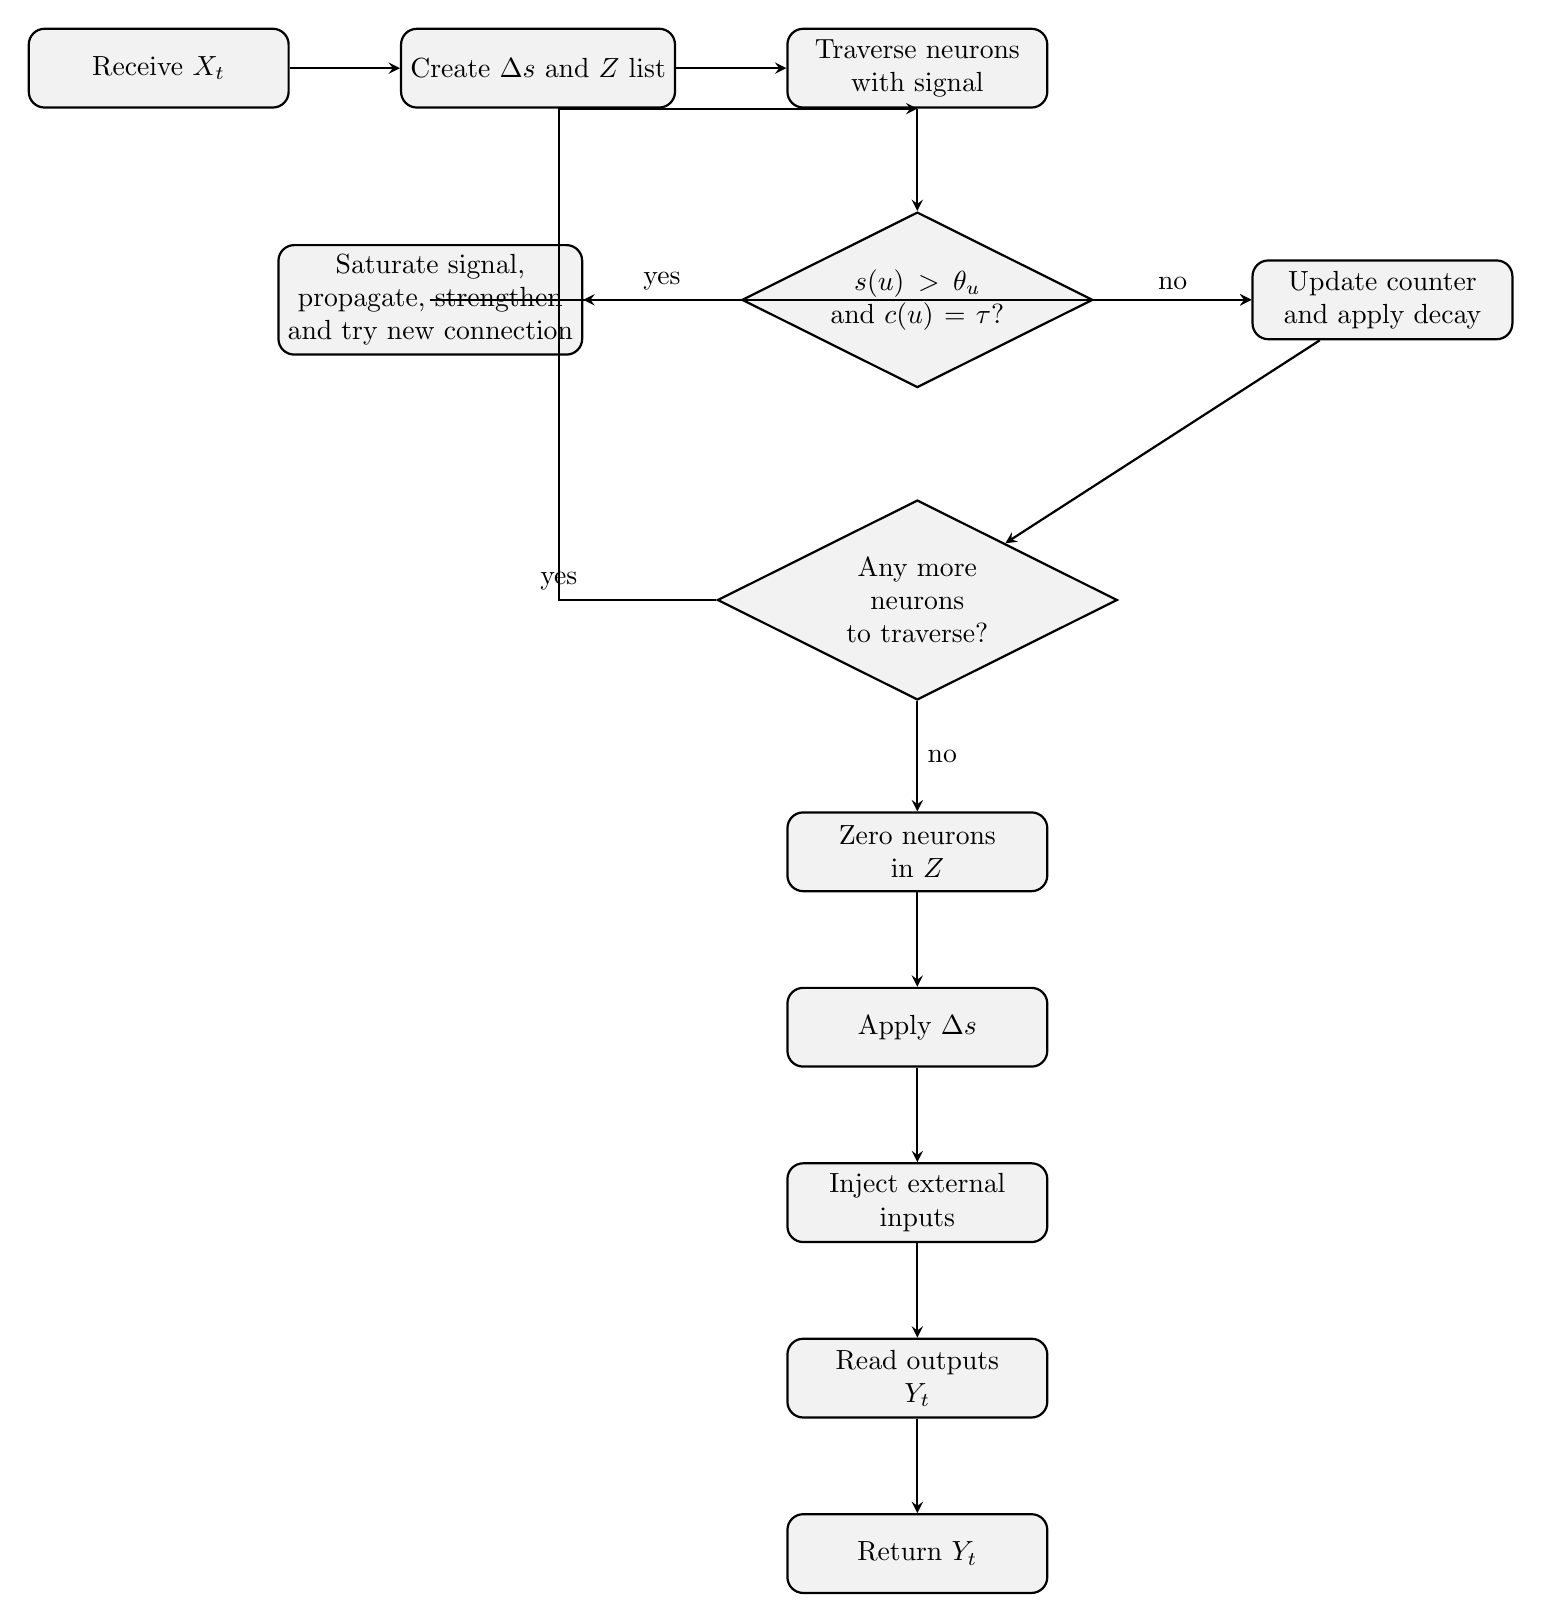
\begin{tikzpicture}[node distance=1.0cm and 1.0cm]
	\node[flowblock] (r1) {Receive $X_t$};
	\node[flowblock, right=1.4cm of r1] (r2) {Create $\Delta s$ and $Z$ list};
	\node[flowblock, right=1.4cm of r2] (r3) {Traverse neurons\\with signal};
	\node[flowdecision, below=1.3cm of r3] (d1) {$s(u)>\theta_u$\\and $c(u)=\tau$?};
	\node[flowblock, left=2.0cm of d1] (r4) {Saturate signal,\\propagate, strengthen\\and try new connection};
	\node[flowblock, right=2.0cm of d1] (r5) {Update counter\\and apply decay};
	\node[flowdecision, below=1.4cm of d1] (d2) {Any more neurons\\to traverse?};
	\node[flowblock, below=1.4cm of d2] (r6) {Zero neurons\\in $Z$};
	\node[flowblock, below=1.2cm of r6] (r7) {Apply $\Delta s$};
	\node[flowblock, below=1.2cm of r7] (r8) {Inject external\\inputs};
	\node[flowblock, below=1.2cm of r8] (r9) {Read outputs\\$Y_t$};
	\node[flowblock, below=1.2cm of r9] (r10) {Return $Y_t$};

	\draw[flowline] (r1) -- (r2);
	\draw[flowline] (r2) -- (r3);
	\draw[flowline] (r3) -- (d1);
	\draw[flowline] (d1) -- node[above]{yes} (r4);
	\draw[flowline] (d1) -- node[above]{no} (r5);
	\draw[flowline] (r4) |- (r5);
	\draw[flowline] (r5) -- (d2);
	\draw[flowline] (d2) -- node[right]{no} (r6);
	\draw[flowline] (r6) -- (r7);
	\draw[flowline] (r7) -- (r8);
	\draw[flowline] (r8) -- (r9);
	\draw[flowline] (r9) -- (r10);
	\draw[flowline] (d2.west) -- ++(-2.0,0) node[above]{yes} |- (r3.south);
\end{tikzpicture}}
\caption{Flowchart of Algorithm 2. Neuronal processing combines internal updating, plasticity, sensory injection, and output readout in a single discrete step.}
\label{fig:fluxo-processamento}
\end{figure}

\section{Offspring rules}

\subsection{Reproductive event}

Reproduction is triggered by the environment when two blobs collide and satisfy the behavioral conditions imposed by the simulation: minimum age, child limit, cooldown, and population cap. When reproduction is requested, the backend receives the identifiers of two parent organisms, say $P_1$ and $P_2$.

If either parent is not registered in the set of live organisms maintained by the backend, the offspring fails. Otherwise, the system tries to generate a child by genetic recombination. In the current prototype, generation is attempted at most twice; if the validity constraints fail repeatedly, no child is returned.

\subsection{Child dimensions}

Let
$$
	(a_1,b_1,c_1),\qquad (a_2,b_2,c_2)
$$
be the parent dimensions. The child dimensions are sampled uniformly from the closed intervals between the parental values:
$$
	a_h\sim\UnifInt(\min(a_1,a_2),\max(a_1,a_2)),
$$
$$
	b_h\sim\UnifInt(\min(b_1,b_2),\max(b_1,b_2)),
$$
$$
	c_h\sim\UnifInt(\min(c_1,c_2),\max(c_1,c_2)).
$$
The number of neurons in the child is
$$
	M_h=a_hb_hc_h.
$$

\subsection{Cut operator}

To recombine blocks of size $L$, define a cut point
$$
	\rho_L\sim\UnifInt(\lfloor0.4L\rfloor,\lfloor0.6L\rfloor).
$$
The cut-based crossover operation is
$$
	\operatorname{cross}(A,B;\rho_L)_r=
	\begin{cases}
		A_r, & r<\rho_L,\\
		B_r, & r\geq\rho_L.
	\end{cases}
$$
The implementation uses this pattern for input genes, output genes, output thresholds, regions, initial connections, probabilities, and internal thresholds, with adaptations when the child has more neurons than the parents.

\subsection{Child inputs}

Choose
$$
	\rho_I\sim\UnifInt(\lfloor0.4N_I\rfloor,\lfloor0.6N_I\rfloor).
$$
The child input gene is
$$
	G_I^h[r]=
	\begin{cases}
		G_I^{P_1}[r], & r<\rho_I,\\
		G_I^{P_2}[r], & r\geq\rho_I.
	\end{cases}
$$
Then each row is reinterpreted in the child's dimensions:
$$
	i_r^h=\Phi_{a_h,b_h,c_h}^{(D)}(G_I^h[r]).
$$
The generation is accepted only if
$$
	\card\{i_1^h,\ldots,i_{N_I}^h\}=N_I.
$$
Otherwise, a new offspring attempt is started.

\subsection{Child outputs}

Similarly,
$$
	\rho_O\sim\UnifInt(\lfloor0.4N_O\rfloor,\lfloor0.6N_O\rfloor),
$$
and
$$
	G_O^h[r]=
	\begin{cases}
		G_O^{P_1}[r], & r<\rho_O,\\
		G_O^{P_2}[r], & r\geq\rho_O.
	\end{cases}
$$
The child output neurons are
$$
	 o_r^h=\Phi_{a_h,b_h,c_h}^{(D)}(G_O^h[r]).
$$
The generation is accepted only if
$$
	\card\{o_1^h,\ldots,o_{N_O}^h\}=N_O
$$
and
$$
	\{o_1^h,\ldots,o_{N_O}^h\}\cap\{i_1^h,\ldots,i_{N_I}^h\}=\varnothing.
$$

\subsection{Child output thresholds}

Choose
$$
	\rho_{O,\theta}\sim\UnifInt(\lfloor0.4N_O\rfloor,\lfloor0.6N_O\rfloor).
$$
Then
$$
	G_{O,\theta}^h[r]=
	\begin{cases}
		G_{O,\theta}^{P_1}[r], & r<\rho_{O,\theta},\\
		G_{O,\theta}^{P_2}[r], & r\geq\rho_{O,\theta}.
	\end{cases}
$$
The phenotypic threshold is again
$$
	\Theta_{o_r^h}^{out,h}=\mu(G_{O,\theta}^h[r]).
$$

\subsection{Child local regions}

The regions are recombined across $M_h$ positions. Choose
$$
	\rho_R\sim\UnifInt(\lfloor0.4M_h\rfloor,\lfloor0.6M_h\rfloor).
$$
For each index $u\in\{0,\ldots,M_h-1\}$,
$$
	G_R^h[u]=
	\begin{cases}
		G_R^{P_1}[u], & u<\rho_R\text{ and }u<M_1,\\
		G_R^{P_2}[u], & u<\rho_R\text{ and }u\geq M_1\text{ and }u<M_2,\\
		\text{random gene}, & u<\rho_R\text{ and no parental gene is available},\\
		G_R^{P_2}[u], & u\geq\rho_R\text{ and }u<M_2,\\
		G_R^{P_1}[u], & u\geq\rho_R\text{ and }u\geq M_2\text{ and }u<M_1,\\
		\text{random gene}, & u\geq\rho_R\text{ and no parental gene is available}.
	\end{cases}
$$
That is: before the cut there is preference for parent $P_1$; after the cut there is preference for parent $P_2$; when the child has neurons beyond the genetic reach of the parents, the gene is filled randomly.

\subsection{Child initial number of connections}

The gene $G_Q^h$ is chosen entirely from one of the parents:
$$
	G_Q^h=
	\begin{cases}
		G_Q^{P_1}, & U>0.5,\\
		G_Q^{P_2}, & U\leq0.5,
	\end{cases}
	\qquad U\sim\operatorname{Uniform}(0,1).
$$
Then
$$
	Q_h=D_{D_4}(G_Q^h)\bmod(M_h-1).
$$

\subsection{Child initial connections}

For each neuron $u$ in the child, choose
$$
	\rho_E\sim\UnifInt(\lfloor0.4Q_h\rfloor,\lfloor0.6Q_h\rfloor).
$$
For each candidate $w\in\{1,\ldots,Q_h\}$, use the preference rule:
$$
	G_E^h[u,w]=
	\begin{cases}
		G_E^{P_1}[u,w], & w<\rho_E\text{ and available},\\
		G_E^{P_2}[u,w], & w<\rho_E\text{ and }P_1\text{ unavailable but }P_2\text{ available},\\
		\text{random gene}, & w<\rho_E\text{ and unavailable in both parents},\\
		G_E^{P_2}[u,w], & w\geq\rho_E\text{ and available},\\
		G_E^{P_1}[u,w], & w\geq\rho_E\text{ and }P_2\text{ unavailable but }P_1\text{ available},\\
		\text{random gene}, & w\geq\rho_E\text{ and unavailable in both parents}.
	\end{cases}
$$
Each candidate word is reinterpreted in the child's dimensions, and the corresponding connection is accepted if it is not duplicated, if the reverse connection does not exist, and if the destination lies inside the local region of the source neuron.

\subsection{Child plasticity probabilities}

Choose
$$
	\rho_P\sim\UnifInt(\lfloor0.4M_h\rfloor,\lfloor0.6M_h\rfloor).
$$
For each neuron $u$,
$$
	G_P^h[u]=
	\begin{cases}
		G_P^{P_1}[u], & u<\rho_P\text{ and available},\\
		G_P^{P_2}[u], & u<\rho_P\text{ and }P_1\text{ unavailable but }P_2\text{ available},\\
		\text{random gene}, & u<\rho_P\text{ and unavailable in both parents},\\
		G_P^{P_2}[u], & u\geq\rho_P\text{ and available},\\
		G_P^{P_1}[u], & u\geq\rho_P\text{ and }P_2\text{ unavailable but }P_1\text{ available},\\
		\text{random gene}, & u\geq\rho_P\text{ and unavailable in both parents}.
	\end{cases}
$$
The phenotype is
$$
	p_u^h=\mu(G_P^h[u]).
$$

\subsection{Child internal thresholds}

The recombination of internal thresholds follows the same rule as the probabilities:
$$
	\rho_\theta\sim\UnifInt(\lfloor0.4M_h\rfloor,\lfloor0.6M_h\rfloor),
$$
with preference for $P_1$ before the cut and for $P_2$ after the cut. The final threshold is
$$
	\theta_u^h=\mu(G_\theta^h[u]).
$$

\subsection{Inherited or generated global parameters}

The decay is inherited entirely from one of the parents:
$$
	G_\delta^h=
	\begin{cases}
		G_\delta^{P_1}, & U>0.5,\\
		G_\delta^{P_2}, & U\leq0.5.
	\end{cases}
$$
The post-firing inactivity is generated again at random:
$$
	G_\tau^h\sim\operatorname{Uniform}(\SigmaGen^{D_2}),
	\qquad
	\tau_h=D_{D_2}(G_\tau^h)+1.
$$
The exponential factor is inherited entirely from one of the parents:
$$
	G_\kappa^h=
	\begin{cases}
		G_\kappa^{P_1}, & U>0.5,\\
		G_\kappa^{P_2}, & U\leq0.5.
	\end{cases}
$$
The reserved gene $G_\omega$ is also inherited entirely from one of the parents:
$$
	G_\omega^h=
	\begin{cases}
		G_\omega^{P_1}, & U>0.5,\\
		G_\omega^{P_2}, & U\leq0.5.
	\end{cases}
$$

\subsection{Offspring algorithm}

Algorithm 3. Offspring generation

\begin{enumerate}
	\item Receive parent identifiers $P_1$ and $P_2$.
	\item If any parent does not exist in the backend, return failure.
	\item Repeat for at most two attempts:
	\begin{enumerate}
		\item sample the child dimensions between the parents' dimensions;
		\item recombine input genes with a cut between $40\%$ and $60\%$;
		\item reinterpret inputs in the child dimensions;
		\item if there is a collision among inputs, restart the attempt;
		\item recombine output genes with a cut between $40\%$ and $60\%$;
		\item reinterpret outputs in the child dimensions;
		\item if there is a collision among outputs or an input--output intersection, restart the attempt;
		\item recombine output thresholds;
		\item recombine local regions, using random genes when the child has neurons without parental correspondence;
		\item inherit the initial number of connections gene from one of the parents;
		\item recombine the initial connection genes for each neuron;
		\item recombine plasticity probabilities;
		\item recombine internal thresholds;
		\item inherit decay, exponential factor, and the reserved weakening gene;
		\item generate the inactivity period randomly;
		\item initialize signals, synaptic strengths, counters, and number of children.
	\end{enumerate}
	\item If an attempt is accepted, return the child.
	\item If all attempts fail, return failure.
\end{enumerate}

\begin{figure}[H]
\centering
\resizebox{\textwidth}{!}{%
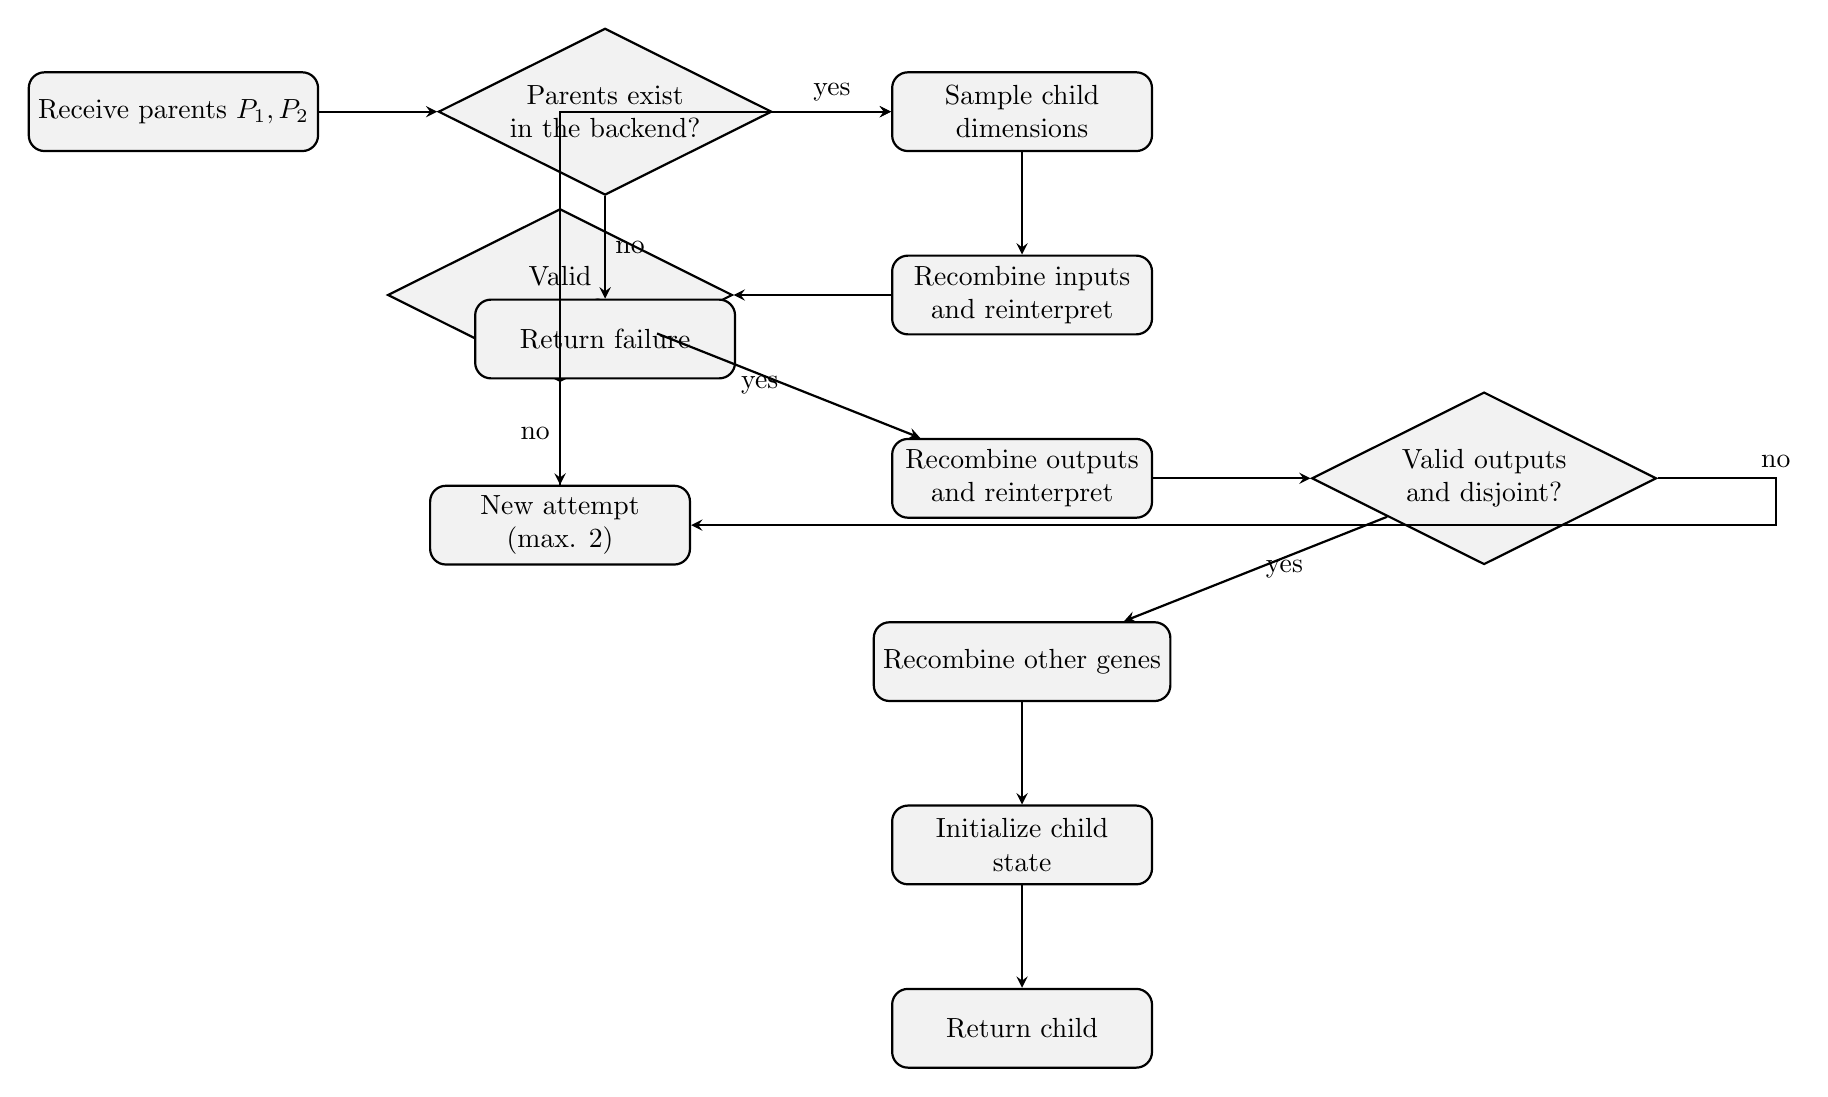
\begin{tikzpicture}[node distance=1.0cm and 1.0cm]
	\node[flowblock] (s1) {Receive parents $P_1,P_2$};
	\node[flowdecision, right=1.5cm of s1] (s2) {Parents exist\\in the backend?};
	\node[flowblock, right=1.5cm of s2] (s3) {Sample child\\dimensions};
	\node[flowblock, below=1.3cm of s3] (s4) {Recombine inputs\\and reinterpret};
	\node[flowdecision, left=2.0cm of s4] (s5) {Valid\\inputs?};
	\node[flowblock, below=1.3cm of s4] (s6) {Recombine outputs\\and reinterpret};
	\node[flowdecision, right=2.0cm of s6] (s7) {Valid outputs\\and disjoint?};
	\node[flowblock, below=1.3cm of s6] (s8) {Recombine other genes};
	\node[flowblock, below=1.3cm of s8] (s9) {Initialize child\\state};
	\node[flowblock, below=1.3cm of s9] (s10) {Return child};
	\node[flowblock, below=1.3cm of s5] (s11) {New attempt\\(max. 2)};
	\node[flowblock, below=1.3cm of s2] (s12) {Return failure};

	\draw[flowline] (s1) -- (s2);
	\draw[flowline] (s2) -- node[above]{yes} (s3);
	\draw[flowline] (s2) -- node[right]{no} (s12);
	\draw[flowline] (s3) -- (s4);
	\draw[flowline] (s4) -- (s5);
	\draw[flowline] (s5) -- node[left]{yes} (s6);
	\draw[flowline] (s5) -- node[left]{no} (s11);
	\draw[flowline] (s6) -- (s7);
	\draw[flowline] (s7) -- node[right]{yes} (s8);
	\draw[flowline] (s7.east) -- ++(1.5,0) node[above]{no} |- (s11.east);
	\draw[flowline] (s8) -- (s9);
	\draw[flowline] (s9) -- (s10);
	\draw[flowline] (s11) |- (s3.west);
\end{tikzpicture}}
\caption{Flowchart of Algorithm 3. The offspring is a recombination with structural validation; whenever the child's inputs or outputs become invalid, a new attempt is made.}
\label{fig:fluxo-offspring}
\end{figure}

\section{Ecology, energy, and selective pressure}

The environment acts as a selection mechanism. Each organism has an energy $E_b(t)$, initialized to $1.0$. Executing actions consumes energy:

\begin{table}[H]
\centering
\caption{Energy costs of the implemented actions.}
\label{tab:energia}
\begin{tabular}{lll}
\toprule
Action & Condition & Cost \\
\midrule
forward movement & $Y^1=1$ & $0.002$ \\
backward movement & $Y^2=1$ and $Y^1\neq1$ & $0.002$ \\
positive rotation & $Y^3=1$ & $0.0015$ \\
negative rotation & $Y^4=1$ and $Y^3\neq1$ & $0.0015$ \\
basal decay & every processed step & $0.001$ \\
reproduction & offspring event & $0.01$ \\
\bottomrule
\end{tabular}
\end{table}

When the organism eats, its energy increases:
$$
	E_b(t+1)=\min\{2.0,E_b(t)+0.5\}.
$$

Reproduction requires a collision between two blobs and the following conditions: minimum age greater than $100$ life steps, reproduction cooldown, maximum number of children per blob, and total population below the allowed maximum. The child is born with initial energy $0.5$.

There is no explicit fitness. Fitness is implicit and ecological:
$$
	\text{effective fitness} \approx \text{survive} + \text{find food} + \text{reproduce}.
$$

\begin{figure}[H]
\centering
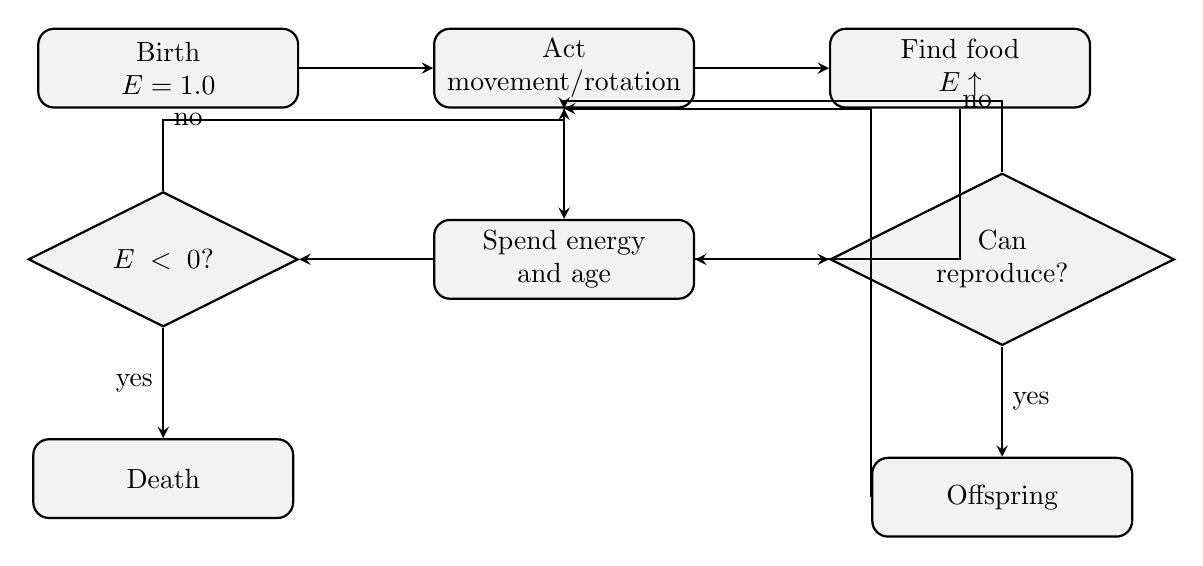
\begin{tikzpicture}[node distance=1.3cm]
	\node[flowblock] (nasc) {Birth\\$E=1.0$};
	\node[flowblock, right=1.7cm of nasc] (agir) {Act\\movement/rotation};
	\node[flowblock, right=1.7cm of agir] (comer) {Find food\\$E\uparrow$};
	\node[flowblock, below=1.4cm of agir] (gastar) {Spend energy\\and age};
	\node[flowdecision, left=1.7cm of gastar] (morre) {$E<0$?};
	\node[flowdecision, right=1.7cm of gastar] (repro) {Can\\reproduce?};
	\node[flowblock, below=1.4cm of morre] (fim) {Death};
	\node[flowblock, below=1.4cm of repro] (filho) {Offspring};
	\draw[flowline] (nasc) -- (agir);
	\draw[flowline] (agir) -- (comer);
	\draw[flowline] (agir) -- (gastar);
	\draw[flowline] (comer) |- (gastar);
	\draw[flowline] (gastar) -- (morre);
	\draw[flowline] (gastar) -- (repro);
	\draw[flowline] (morre) -- node[left]{yes} (fim);
	\draw[flowline] (morre.north) -- ++(0,0.9) node[right]{no} -| (agir.south);
	\draw[flowline] (repro) -- node[right]{yes} (filho);
	\draw[flowline] (repro.north) -- ++(0,0.9) node[left]{no} -| (agir.south);
	\draw[flowline] (filho.west) |- (agir.south);
\end{tikzpicture}
\caption{Simplified ecological cycle of the blob: act, spend energy, find food, and eventually reproduce or die.}
\label{fig:ciclo-ecologico}
\end{figure}

\section{Implementation methodology}

\subsection{Overall architecture}

The implementation is divided into two parts:

\begin{enumerate}
	\item \textbf{Godot frontend:} responsible for the two-dimensional environment, physics, visualization, collisions, food, energy, input collection, and output application.
	\item \textbf{Python backend:} responsible for brain generation, genome storage, neuronal processing, plasticity, offspring, and communication via WebSocket.
\end{enumerate}

Communication occurs through a local WebSocket at the address
\begin{center}
\texttt{ws://127.0.0.1:8000/ws}
\end{center}
The backend uses FastAPI and Uvicorn. The frontend uses Godot's \texttt{WebSocketPeer}.

\begin{figure}[H]
\centering
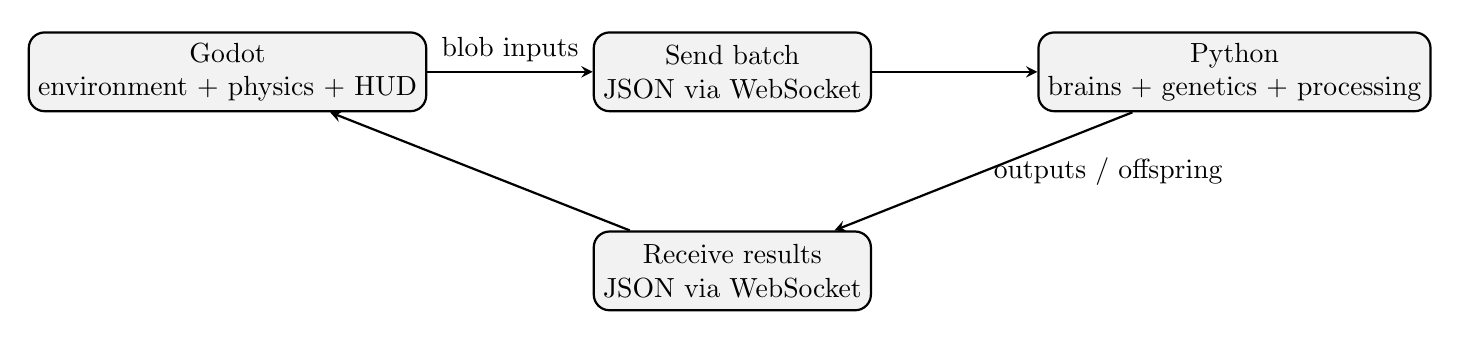
\begin{tikzpicture}[node distance=1.6cm]
	\node[flowblock] (godot) {Godot\\environment + physics + HUD};
	\node[flowblock, right=2.1cm of godot] (ws1) {Send batch\\JSON via WebSocket};
	\node[flowblock, right=2.1cm of ws1] (python) {Python\\brains + genetics + processing};
	\node[flowblock, below=1.5cm of ws1] (ws2) {Receive results\\JSON via WebSocket};
	\draw[flowline] (godot) -- node[above]{blob inputs} (ws1);
	\draw[flowline] (ws1) -- (python);
	\draw[flowline] (python) -- node[right]{outputs / offspring} (ws2);
	\draw[flowline] (ws2) -- (godot);
\end{tikzpicture}
\caption{Logical-operational architecture of the implementation. Godot controls the environment and Python controls the brain logic; both communicate in batches via WebSocket.}
\label{fig:arquitetura}
\end{figure}

\subsection{Communication protocol}

Communication is done in batches. The frontend sends a JSON message of the form
\begin{center}
\texttt{\{"batch": [requests]\}}
\end{center}
Each request has a \texttt{npc\_action} field. The main actions are:

\begin{table}[H]
\centering
\caption{Actions supported by the backend.}
\label{tab:websocket}
\begin{tabular}{ll}
\toprule
Action & Function \\
\midrule
\texttt{gen\_brain} & generate a new brain for a blob \\
\texttt{process} & process inputs and return outputs \\
\texttt{offspring} & generate an offspring from two parents \\
\bottomrule
\end{tabular}
\end{table}

The backend response has the form
\begin{center}
\texttt{\{"results": [results]\}}
\end{center}
For processing, each result includes the blob identifier, output vector, current number of connections, and maximum possible brain size.

\subsection{Implemented inputs}

The blob input vector has $16$ components:
$$
	X=(X_1,\ldots,X_{16}).
$$
In the current implementation:
$$
\begin{aligned}
X_1 &= \max(0,v_x),&
X_2 &= \max(0,-v_x),\\
X_3 &= \max(0,v_y),&
X_4 &= \max(0,-v_y),\\
X_5 &= \max(0,\omega),&
X_6 &= \max(0,-\omega),\\
X_7 &= |\rho/(2\pi)|,&
X_8 &= E_b,\\
X_9 &= \frac{1}{1+E_b},&
X_{10} &= \text{food-proximity counter},\\
X_{11} &= \text{collision indicator},&
X_{12} &= \min(10,100/d),\\
X_{13} &= Y_{t-1}^1,&
X_{14} &= Y_{t-1}^2,\\
X_{15} &= Y_{t-1}^3,&
X_{16} &= Y_{t-1}^4.
\end{aligned}
$$
Here $v_x,v_y$ are linear velocity components, $\omega$ is the angular velocity, $\rho$ is the current rotation of the blob, $E_b$ is the energy, and $d$ is the distance to a detected food item.

The four previous outputs are fed back as inputs, producing a short-term behavioral memory in the organism--environment coupling.

\begin{table}[H]
\centering
\caption{Didactic summary of the $16$ inputs.}
\label{tab:inputs-resumo}
\begin{tabular}{cl}
\toprule
Input & Description \\
\midrule
$X_1,X_2$ & positive and negative horizontal velocity \\
$X_3,X_4$ & positive and negative vertical velocity \\
$X_5,X_6$ & positive and negative angular velocity \\
$X_7$ & normalized rotation \\
$X_8,X_9$ & energy and regularized inverse energy \\
$X_{10},X_{12}$ & proximity and inverse distance to food \\
$X_{11}$ & collision \\
$X_{13},\ldots,X_{16}$ & previous-step outputs \\
\bottomrule
\end{tabular}
\end{table}

\subsection{Implemented outputs}

The binary outputs control body and energy:

\begin{enumerate}
	\item $Y^1=1$: defines forward linear velocity in the direction of the current rotation.
	\item $Y^2=1$: defines backward linear velocity relative to the rotation.
	\item $Y^3=1$: defines positive angular rotation.
	\item $Y^4=1$: defines negative angular rotation.
\end{enumerate}

The physical body of the blob is a gravity-free \texttt{RigidBody2D} with linear and angular damping. The scene contains static walls that delimit the environment.

\subsection{Food and environmental sensors}

Each food item has two detection areas:

\begin{enumerate}
	\item a larger area, which indicates proximity and provides distance;
	\item a smaller area, which represents food consumption.
\end{enumerate}

When the blob enters the larger area, it receives a proximity signal and inverse distance. When it enters the smaller area, the food is removed from the scene and the blob's energy increases. New food items are periodically added to the environment.

\subsection{Computational economy}

Processing every brain in every frame can become costly. For this reason, the backend uses a cost-saving strategy: the blob with identifier \texttt{blob\_0} is always processed, while the others are processed in subsets defined by the numeric identifier modulo $5$. Thus, each request processes only part of the population, reducing the cost per frame.

The \texttt{blob\_0} is also used as a reference organism for logging neuronal activity. In the frontend, its energy is kept at $1.0$ to prevent it from dying before the simulation ends.

\subsection{Histories and visualization}

The backend keeps two histories in memory:

\begin{enumerate}
	\item neuronal signal history;
	\item history of the number of connections per blob.
\end{enumerate}

The post-processing visualization script uses Plotly to generate a three-dimensional animation of neuronal activity and a time series of the number of connections. These tools are important for evaluating the structural and dynamic evolution of the brains, even though the current prototype version must ensure consistency between the saved history format and the format expected by the visualization.

\begin{figure}[H]
\centering
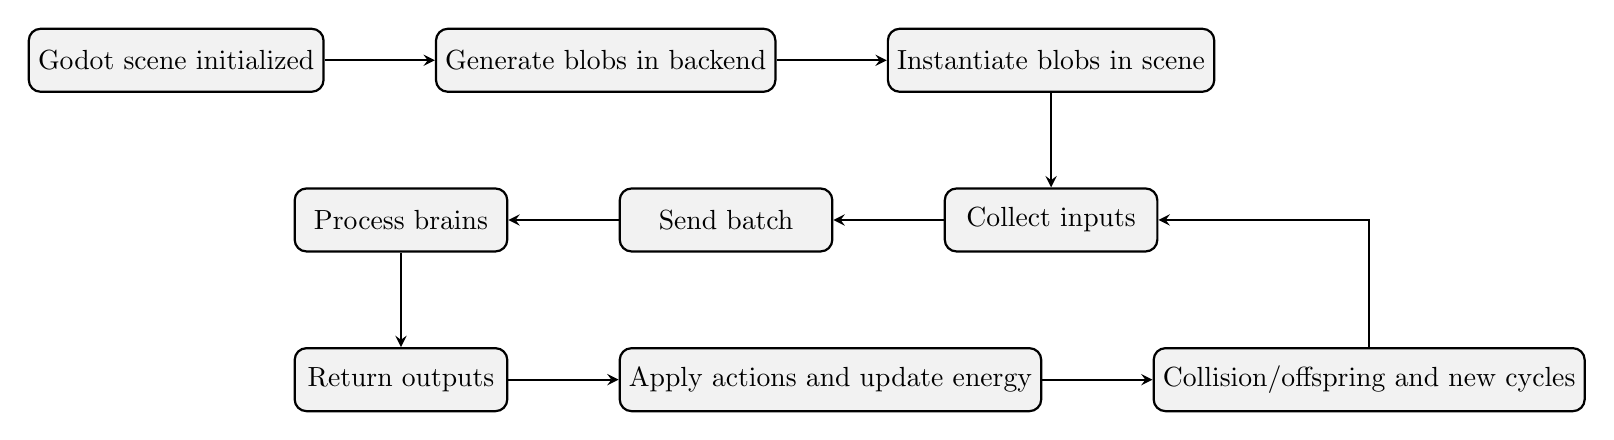
\begin{tikzpicture}[node distance=1.4cm]
	\node[flowsmall] (f1) {Godot scene initialized};
	\node[flowsmall, right=1.4cm of f1] (f2) {Generate blobs in backend};
	\node[flowsmall, right=1.4cm of f2] (f3) {Instantiate blobs in scene};
	\node[flowsmall, below=1.2cm of f3] (f4) {Collect inputs};
	\node[flowsmall, left=1.4cm of f4] (f5) {Send batch};
	\node[flowsmall, left=1.4cm of f5] (f6) {Process brains};
	\node[flowsmall, below=1.2cm of f6] (f7) {Return outputs};
	\node[flowsmall, right=1.4cm of f7] (f8) {Apply actions and update energy};
	\node[flowsmall, right=1.4cm of f8] (f9) {Collision/offspring and new cycles};
	\draw[flowline] (f1) -- (f2);
	\draw[flowline] (f2) -- (f3);
	\draw[flowline] (f3) -- (f4);
	\draw[flowline] (f4) -- (f5);
	\draw[flowline] (f5) -- (f6);
	\draw[flowline] (f6) -- (f7);
	\draw[flowline] (f7) -- (f8);
	\draw[flowline] (f8) -- (f9);
	\draw[flowline] (f9.north) |- (f4.east);
\end{tikzpicture}
\caption{Summary of the operational cycle of the implementation. The system alternates between perception, brain processing, action, and environmental update.}
\label{fig:ciclo-operacional}
\end{figure}

\section{Discussion}

The proposed model clearly separates three levels of adaptation:

\begin{enumerate}
	\item \textbf{Genetic adaptation:} brain structures are generated and recombined by discrete genes.
	\item \textbf{Individual adaptation:} internal connections can be created and weakened during the organism's life.
	\item \textbf{Ecological adaptation:} the environment selects organisms by survival, feeding, and reproduction.
\end{enumerate}

The absence of layers and of an explicit loss function makes the model less controllable, but also more open. Useful behaviors are not imposed by direct engineering; they must emerge from combinations of topology, signals, plasticity, and selective pressure. This openness is precisely the point of interest of the prototype.

There are, however, important limitations. The simulation still lacks consolidated metrics for population performance, explicit point-mutation mechanisms in offspring, statistical lineage analysis, and comparison with baselines. In addition, some genes already exist in the structure, such as the weakened period, but are not yet used in the dynamics. Such elements should be treated as natural extensions of the model.

\begin{table}[H]
\centering
\caption{Summary of the prototype's hypotheses and implications.}
\label{tab:hipoteses}
\begin{tabular}{p{5.1cm}p{8.9cm}}
\toprule
Modeling hypothesis & Experimental implication \\
\midrule
Layer-free topology & enables emergent recurrence and local geometry \\
Discrete genome with indirect mapping & favors structural diversity and rejection of invalid brains \\
Plasticity during life & separates ontogenetic adaptation from evolutionary adaptation \\
Selection without explicit fitness & shifts the problem to the environment's ecology \\
Distributed backend processing & makes possible brains that are more expensive than full execution inside the graphical engine \\
\bottomrule
\end{tabular}
\end{table}

\section{Conclusion}

This article formalized a prototype of artificial neuronal evolution simulation. Each organism has a brain defined by a three-dimensional mesh of neurons, directional connections, thresholds, local connectivity regions, exponential response, structural plasticity, and selective weakening of internal connections. The initial generation of brains is genetic, reproduction occurs through recombination of parental genes, and selection is determined by the environment.

The model does not aim to replace traditional artificial neural networks, but rather to explore an alternative regime of artificial intelligence based on organisms, ecology, plasticity, and evolution. The natural next step is to instrument the histories better, introduce lineage metrics, test different mutation rules, and evaluate whether more adapted neuronal structures emerge robustly under different environmental configurations.

\end{document}
